\documentclass[11pt]{beamer}
\usepackage{graphicx}
\usepackage{longtable}
\usepackage{wrapfig}
\usepackage{rotating}
\usepackage[normalem]{ulem}
\usepackage{amsmath}
\usepackage{amssymb}
\usepackage{capt-of}
\usepackage{hyperref}
\institute{Università di Siena}
\usepackage{localheader}
\usepackage{tikz}
\usepackage{booktabs}
\usepackage{setspace}
\usepackage{quoting}
\usepackage[italian]{babel}
\usepackage{fancybox}
\usetheme{default}
\author{Massimo D'Antoni}
\date{2023-2024}
\title{La spesa previdenziale}
\subtitle{Scienza delle Finanze}
\hypersetup{
 pdfauthor={Massimo D'Antoni},
 pdftitle={La spesa previdenziale},
 pdflang={Italian}}
\begin{document}

\maketitle

\section{L'intervento pubblico in ambito pensionistico}

%%%%%%%%%%%%%%%%%%%%%%%%%%%%%%%%%%%%%%%%%%%%%%
\begin{frame}{Il ruolo dello Stato in ambito pensionistico}
\begin{itemize}
\item Guardando all'esperienza delle economie avanzate:
\begin{itemize}
\item in molti caso lo Stato assume una responsabilità diretta nella fornitura di
pensioni
\item quando le pensioni sono fornite da fondi pensionistici privati sono
comunque previsti l'obbligo di versamento di contributi e incentivi
fiscali a chi mette il proprio risparmio in fondi pensione. Inoltre,
regolamentazione dei fondi pensione e garanzie pubbliche
\end{itemize}

\item Da un punto di vista individuale, la pensione svolge una funzione di
\alert{risparmio} e di \alert{assicurazione}:
\begin{itemize}
\item risparmio a lungo termine, finalizzato al mantenimento del tenore di vita
dopo la cessazione dell'attività lavorativa
\item assicurazione rispetto alla durata della propria vita
\end{itemize}

\item Accanto a tale funzione \alert{previdenziale} e \alert{assicurativa}, il sistema
pensionistico, quando gestito dallo Stato, può svolgere anche una funzione
\alert{assistenziale} (contrasto a situazioni di povertà) e perseguire finalità
\alert{redistributive}
\end{itemize}
\end{frame}

%%%%%%%%%%%%%%%%%%%%%%%%%%%%%%%%%%%%%%%%%%%%%%
\begin{frame}{La funzione assicurativa e la conversione del risparmio in rendita}
\begin{itemize}
\item Data l'incertezza sulla durata della vita residua del pensionato, se la
finalità è il finanziamento dei consumi in età anziana è \alert{sempre}
conveniente convertire il risparmio in rendita (\emph{annuity}).
\item Ipotesi: risparmio 100€ con rendimento 20\%
\begin{itemize}
\item titolo X: pagamento incondizionato di 120€ a scadenza
\item titolo Y: pagamento di 200€ a scadenza condizionato al fatto che
l'individuo sia in vita (probabilità 60\%)
\item per il fondo/assicuratore i due titoli sono equivalenti
\item per il sottoscrittore, conviene il titolo Y, perché se l'individuo non è
in vita\ldots{} non consuma!
\end{itemize}
\item La conclusione vale anche in presenza di eredità: in questo caso conviene
scegliere il titolo X per la quota da destinare agli eredi e il titolo Y per
la quota che finanzia il consumo
\end{itemize}
\end{frame}

%%%%%%%%%%%%%%%%%%%%%%%%%%%%%%%%%%%%%%%%%%%%%%
\begin{frame}{Come si può giustificare l'intervento dello Stato /2}
\begin{itemize}
\item Per quale motivo di ritiene necessaria l'introduzione di un obbligo di
versamento di contributi e un obbligo di conversione del risparmio in una
rendita, se tale scelta è ottimale per l'individuo?
\item \alert{Miopia}: l'individuo potrebbe non valutare correttamente le proprie
necessità future.
\begin{itemize}
\item Rischio di «paternalismo»
\end{itemize}
\item Molti individui riconoscono \emph{ex post} di non aver risparmiato abbastanza.
\item \alert{Procrastinazione}: l'individuo, pur riconoscendo le proprie necessità
future, tende a procrastinare l'avvio di un piano di risparmio («risparmio a
partire da domani»).
\begin{itemize}
\item Gli economisti hanno studiato i casi di preferenze che manifestano questo
tipo di «incoerenza temporale»
\item L'imposizione di un obbligo in questo caso è riconosciuto dall'individuo
come qualcosa nel proprio interesse, uno strumento per vincolare il
proprio comportamento.
\item In certi casi è sufficiente intervenire sulle scelte «di /default/»,
prevedendo degli automatismi nelle scelte individuali.
\end{itemize}
\end{itemize}
\end{frame}


%%%%%%%%%%%%%%%%%%%%%%%%%%%%%%%%%%%%%%%%%%%%%%
\begin{frame}{Come si può giustificare l'intervento dello Stato /2}
\begin{itemize}
\item Sul «lato offerta», possono esserci carenze nell'offerta di strumenti
finanziari adeguati
\begin{itemize}
\item Era certamente così in origine, ma è ancora una spiegazione adeguata?
\item La regolazione dei mercati finanziari può limitare alcuni rischi.
\end{itemize}
\item La scarsa propensione a convertire il capitale risparmiato in rendita può
spiegarci con:
\begin{itemize}
\item l'incapacità dell'individuo di comprendere il vantaggio della rendita
\item la \alert{selezione avversa}, quando gli individui hanno diverse aspettative di
durata della vita residua e c'è informazione asimmetrica
\end{itemize}
\item L'obbligo è stato giustificato anche con l'aspettativa dell'individuo di
essere comunque assistito dalla collettività («dilemma del samaritano»)
\begin{itemize}
\item La spiegazione può valere per individui con reddito basso che non
risparmiano, ma non sembra avere valenza generale
\end{itemize}
\item Altre ragioni dell'intervento pubblico hanno a che vedere con
l'organizzazione dei sistemi pensionistici (ripartizione) e con il
perseguimento di ulteriori finalità (ad es. redistributive)
\end{itemize}
\end{frame}

%%%%%%%%%%%%%%%%%%%%%%%%%%%%%%%%%%%%%%%%%%%%%%
\begin{frame}{Evoluzione storica dei sistemi pensionistici}
\begin{itemize}
\item La prima modalità di sostegno agli anziani: nell'ambito della famiglia i
figli mantengono i genitori
\item Organizzazioni mutualistiche e altre associazioni volontarie con lo sviluppo
della società industriale
\item Il coinvolgimento dello Stato è richiesto per le situazioni di insolvenza e
per insufficienza delle soluzioni volontaristiche. Esso comporta
\begin{itemize}
\item introduzioni di obblighi di versamento
\item garanzia sul rendimento minimo
\end{itemize}
\item Germania: nel 1889 (Bismark) prima pensione obbligatoria di tipo
contributivo
\item Approccio alternativo (soprattutto nei paesi anglosassoni): una pensione
minima soggetta a "prova dei mezzi". In Danimarca (1891), Nuova Zelanda
(1898), Australia and Regno Unito (1908), Canada (1927)
\item USA: negli anni 1920 sistema \emph{means-tested} in molti stati. Nel 1935 (New
Deal) introdotta l'OASDI (Old Age Survivors \& Disability Insurance), meglio
nota come \emph{social security}
\item l'espansione dei sistemi di sicurezza sociale si ha soprattutto dopo la II
GM
\end{itemize}
\end{frame}

%%%%%%%%%%%%%%%%%%%%%%%%%%%%%%%%%%%%%%%%%%%%%%
\begin{frame}{In Italia: la creazione del sistema pensionistico}
\begin{columns}
\begin{column}{.5\columnwidth}
\fontsize{10}{10}\selectfont
\begin{description}
\item[{1898}] previdenza \emph{volontaria} per i dipendenti privati, che dà diritto a
rendita vitalizia a partire dai 65 anni, calcolata come capitalizzazione dei
contributi
\item[{1919}] \emph{obbligo} di assicurazione per invalidità e vecchiaia a tutti i
dipendenti privati con retribuzione inferiore a L.800 mensili. Età legale di
pensionamento a 65 anni per uomini e donne.
\item[{1933}] nasce l'INPS (al tempo si chiamava INPFS)
\item[{1939}] pensione di reversibilità ai superstiti; età pensionabile a 60 anni
per uomini, 55 per donne
\item[{1945}] a causa dell'inflazione bellica, si passa alla ripartizione; la
capitalizzazione resta residuale
\item[{1952}] integrazione al minimo delle pensioni
\end{description}
\end{column}
\begin{column}{.5\columnwidth}
\fontsize{10}{10}\selectfont
\begin{description}
\item[{1957-66}] assicurazione obbligatoria per coltivatori, mezzadri e coloni,
artigiani e commercianti
\item[{1965}] introduzione della pensione sociale e la pensione di anzianità (chi
ha 35 anni di contribuzione prescindendo dall'età anagrafica)
\item[{1969}] abbandono definitivo della capitalizzazione; estensione della
pensione sociale a tutti i cittadini anziani privi di qualsiasi reddito
\item[{1975}] pensione agganciata ai salari dell'industria; pensione fino all'80\%
dell'ultima retribuzione
\item[{1981}] allargato su vasta scala l'istituto del prepensionamento
\item[{1990}] riforma della pensione per autonomi, calcolata in modo analogo ai
dipendenti
\item[{(continua)}] 
\end{description}
\vfill
\end{column}
\end{columns}
\end{frame}
%%%%%%%%%%%%%%%%%%%%%%%%%%%%%%%%%%%%%%%%%%%%%%
\begin{frame}{Alcune utili schematizzazioni: "livelli" o "pilastri"}
I tre «livelli» o «pilastri» nella classificazione OCSE:
\begin{enumerate}
\item interventi finalizzati a contrastare la povertà in età anziana garantendo
un minimo standard di vita a tutti i pensionati (pensione di base, minimo
pensionistico, interventi assistenziali)
\item forme di pensione, pubbliche o private obbligatorie o «quasi-obbligatorie»,
il cui importo è rapportato alla retribuzione dell’individuo
(\emph{earning-related})
\item piani pensionistici volontari, gestiti solitamente da fondi privati; la
funzione è quella di garantire uno spazio di scelta individuale
\end{enumerate}

Il livello 1 è pubblico, il 3 è privato. Il livello 2, la componente
quantitativamente più rilevante, può essere organizzata in vari modi. Le differenze riguardano:
\begin{itemize}
\item la presenza o meno di un fondo di attività patrimoniali
\item la formula di calcolo delle prestazioni
\end{itemize}
\end{frame}

\section{L'organizzazione dei sistemi pensionistici}
%%%%%%%%%%%%%%%%%%%%%%%%%%%%%%%%%%%%%%%%%%%%%%
\begin{frame}{Due "famiglie" di sistemi pensionistici}
\begin{itemize}
\item \alert{Sistema a capitalizzazione} (\emph{Fully funded}): pensione futura garantita
dalla titolarità di attività finanziarie accumulate in precedenza, che viene
convertita in una rendita perpetua al momento del pensionamento
\item \alert{Sistema a ripartizione} (\emph{Pas-as-you-go}): pensione futura garantita dai
contributi della popolazione attiva (richiede un patto intergenerazionale e
quindi un'autorità pubblica che può garantirlo: la garanzia è una promessa
dello Stato)
\item Un sistema pubblico può essere parzialmente o totalmente a capitalizzazione
(quindi la distinzione capitalizzazione/ripartizione non coincide con quella
privato/pubblico)
\item Comunque sia organizzato, il sistema determina l'allocazione di una parte
delle risorse prodotte dalla collettività alla popolazione
inattiva:
\begin{itemize}
\item senza il contributo della popolazione attiva, impossibile garantire la
pensione
\item l'invecchiamento della popolazione pone dunque un problema
indipendentemente dalla modalità di organizzazione del sistema
\end{itemize}
\end{itemize}
\end{frame}

%%%%%%%%%%%%%%%%%%%%%%%%%%%%%%%%%%%%%%%%%%%%%%
\begin{frame}{Capitalizzazione e ripartizione}
\begin{columns}
\begin{column}{.5\columnwidth}
\begin{center}
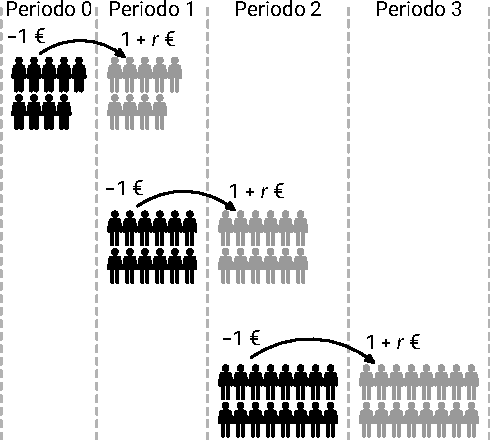
\includegraphics[width=\textwidth]{./figure/olg-capitalizzazione.pdf}
\end{center}

\fontsize{11}{12}\selectfont
Con la \alert{capitalizzazione} i contributi di ciascuna generazione, investiti in
attività reali o finanziarie, finanzieranno le pensioni della stessa
generazione.
\end{column}

\begin{column}{.5\columnwidth}
\begin{center}
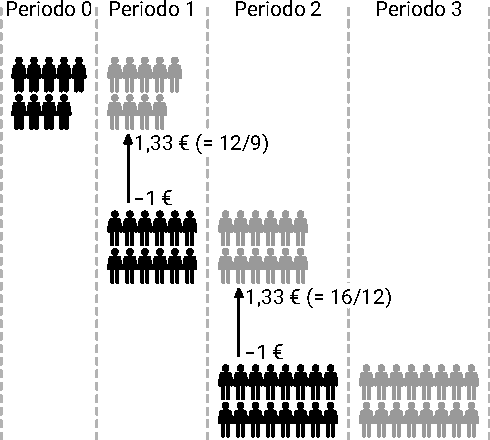
\includegraphics[width=\textwidth]{./figure/olg-ripartizione.pdf}
\end{center}

\fontsize{11}{12}\selectfont

Con la \alert{ripartizione} i contributi di ciascuna generazione attiva finanziano
le pensioni della generazione corrente di anziani.
\bigskip
\end{column}
\end{columns}
\end{frame}

%%%%%%%%%%%%%%%%%%%%%%%%%%%%%%%%%%%%%%%%%%%%%%
\begin{frame}{Il "rendimento" di un sistema pensionistico /1}
\begin{itemize}
\item Il rendimento è dato dal rapporto tra beneficio pensionistico e
versamenti. Per la generazione $i$, ipotizzando per semplicità due periodi:
\begin{equation*}
  \text{rendimento del sistema pensionistico} = \frac{p_i}{t z_i}-1
\end{equation*}
dove $p_i$ è la pensione futura media della generazione $i$, $z_i$ il
salario medio e $t$ l'aliquota contributiva.
\item Nel caso di un sistema a \alert{capitalizzazione}, abbiamo $p_i=(1+r_i)tz_i$, con
$r_i$ rendimento medio ottenibile sui mercati finanziari. Dunque:
\begin{equation*}
  \text{rendimento} = r_i
\end{equation*}
\end{itemize}
\end{frame}

%%%%%%%%%%%%%%%%%%%%%%%%%%%%%%%%%%%%%%%%%%%%%%
\begin{frame}{Il "rendimento" di un sistema pensionistico /2}
\begin{itemize}
\item Anche nel caso di un sistema a \alert{ripartizione}, benché i contributi versati
non vengono investiti, possiamo calcolare il rendimento che tale sistema
garantisce \alert{in media} a un individuo della generazione $i$.
\item Ipotizzando che il sistema sia in equilibrio finanziario abbiamo, con $N_i$
numerosità della generazione $i$: $$N_ip_i=N_{i+1}tz_{i+1}
  \quad\implies\quad p_i=t(N_{i+1}/N_i)z_{i+1}.$$
\item Pertanto:
\begin{equation*}\begin{split}
\text{rendimento}&=(N_{i+1}/N_{i})(z_{i+1}/z_{i})-1\\
&=(1+m)(1+n)-1\\ &\simeq n+m.
\end{split}
\end{equation*}
dove $n$ è il tasso di crescita della forza lavoro e $m$ è il tasso di
crescita dei salari, che si suppone siano allineati alla produttività.
\item Visto che $Y_i=(Y_i/N_i)\cdot N_i$, abbiamo $n+m=g$, dove $g$ è il tasso di
crescita dell'economia.
\end{itemize}
\end{frame}


%%%%%%%%%%%%%%%%%%%%%%%%%%%%%%%%%%%%%%%%%%%%%%
\begin{frame}{Le "formule" di calcolo della pensione}
\begin{itemize}
\item \alert{Contribuzione definita}: corrispondenza attuariale tra contributi versati e prestazioni
$$ P = \delta \cdot MC $$
\item \alert{Prestazione definita}: pensione determinata sulla base delle retribuzioni (solitamente quelle finali) in modo da rendere prevedibile il \alert{tasso di rimpiazzo} 
$$ P = \beta\cdot RP $$
\item Nei sistemi a capitalizzazione sempre più frequente il metodo a contribuzione definita
\item Nei sistemi a ripartizione tradizionalmente prevalente la prestazione definita ("retributivo")
\item Recentemente, nei sistemi a ripartizione, \alert{Contribuzione definita nozionale}
("contributivo"), che "imita" il funzionamento dei fondi a capitalizzazione
e contribuzione definita
\item \alert{Sistemi "a punti"} (es. Germania): in base alla retribuzione si guadagnano
"punti" che sono poi convertiti in pensione
\end{itemize}
\end{frame}

%%%%%%%%%%%%%%%%%%%%%%%%%%%%%%%%%%%%%%%%%%%%%%
\begin{frame}{Il sistema retributivo}
\begin{itemize}
\item Il sistema retributivo vigente in Italia prima della sua sostituzione con il
sistema contributivo, prevedeva:
$$ P = \beta \cdot RP$$
\begin{itemize}
\item $\beta$ pari agli anni di contribuzione $\times$ aliquota massima del 2\%
\item RP determinato come media delle ultime retribuzioni
\end{itemize}
\item Dopo la riforma Dini (1995) applicato integralmente ai lavoratori con almeno
18 anni di contribuzione nel 1995, \emph{pro rata} per i contributi versati
prima del 1995 per tutti gli altri
\item Il \emph{pro rata} è stato esteso a tutti i lavoratori dal 2012.
\end{itemize}
\end{frame}

%%%%%%%%%%%%%%%%%%%%%%%%%%%%%%%%%%%%%%%%%%%%%%
\begin{frame}{Il sistema contributivo}
\begin{itemize}
\item Il montante contributivo:
\begin{equation*}
  \begin{split} MC &= tw_1(1+g)^{L-1}+tw_2(1+g)^{L-2}+\\
  &\quad\dots+tw_{L-1}(1+g)+tw_L.\\ &= t\sum_{i=1}^Lw_i(1+g)^{L-i}
  \end{split}
\end{equation*}
\item La conversione in rendita:
\begin{equation*}
  \begin{split}
  MC &= \frac{P}{1+g}+\frac{P}{(1+g)^2}+
  \dots + \frac{P}{(1+g)^{T-L}} \\
  &=\sum_{i=1}^{T-L}\left(\frac{1}{1+g}\right)^i P
   = \frac{1}{g}\left[1-\left(\frac{1}{1+g}\right)^{T-L}\right] P
    \end{split}
\end{equation*}
da cui, visto che $MC=(1/\delta) P$, otteniamo:
\begin{equation*} \delta =
 \frac{g}{\left[1-\left(\frac{1}{1+g}\right)^{T-L}\right]}.
\end{equation*}
\end{itemize}
\end{frame}


%%%%%%%%%%%%%%%%%%%%%%%%%%%%%%%%%%%%%%%%%%%%%%
\begin{frame}{Il sistema contributivo italiano}
\begin{itemize}
\item Il tasso $g$ è il tasso di crescita del PIL (media mobile quinquennale). In
altri paesi si fa riferimento al tasso di crescita del monte salari.
\item Il coefficiente $\delta$ dipende dall'età e viene periodicamente aggiornato
sulla base dei dati demografici:
\begin{center}\small
  \begin{tabular}{lcc}
  \toprule
  Età di uscita & $1/\delta$ & $\delta$ \\
  \midrule 57 & 23,892 & 4,186\% \\
  60 & 22,149 & 4,515\% \\
  63 & 20,366 & 4,910\% \\
  65 & 19,157 & 5,220\% \\
  68 & 17,324 & 5,772\% \\
  71 & 15,465 & 6,466\% \\
  \bottomrule
\end{tabular} \vspace{1pt}
\end{center}
\end{itemize}
\end{frame}

%%%%%%%%%%%%%%%%%%%%%%%%%%%%%%%%%%%%%%%%%%%%%%
\begin{frame}{L'organizzazione del secondo pilastro}
\begin{figure}[htbp]
\centering
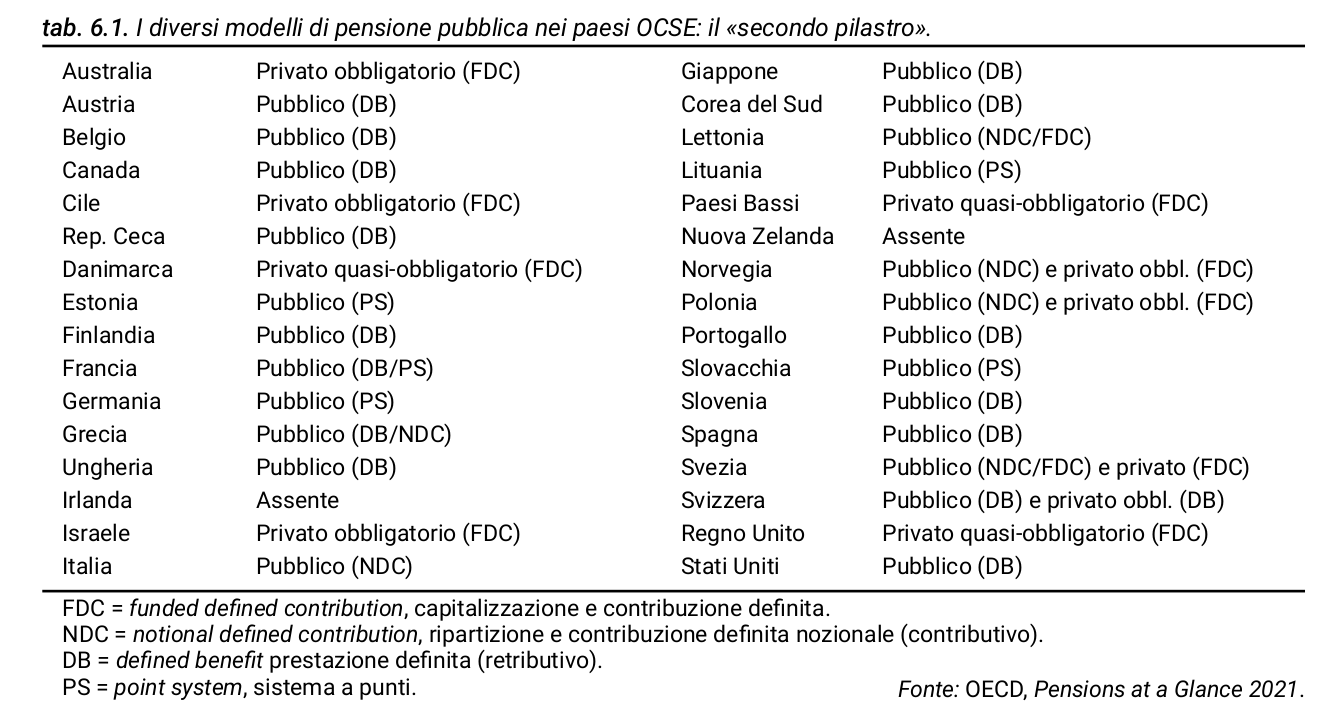
\includegraphics[width=\textwidth]{./figure/secondo-pilastro.png}
\end{figure}
\end{frame}

%%%%%%%%%%%%%%%%%%%%%%%%%%%%%%%%%%%%%%%%%%%%%%
\begin{frame}{La spesa pensionistica}
\begin{figure}[htbp]
\centering
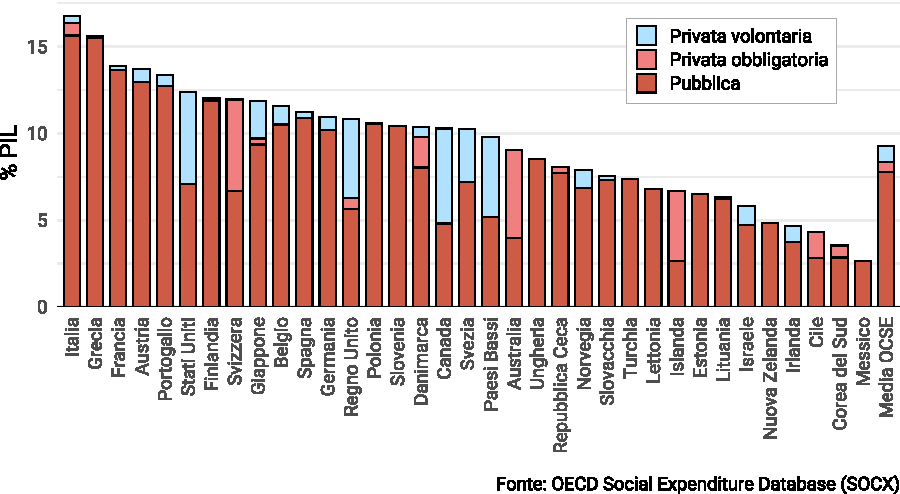
\includegraphics[width=\textwidth]{./figure/pensioni-OECD-publico-privato-2017-color.pdf}
\end{figure}
\end{frame}

%%%%%%%%%%%%%%%%%%%%%%%%%%%%%%%%%%%%%%%%%%%%%%
\begin{frame}{Spesa pubblica in pensioni lorda/netta}
\begin{figure}[htbp]
\centering
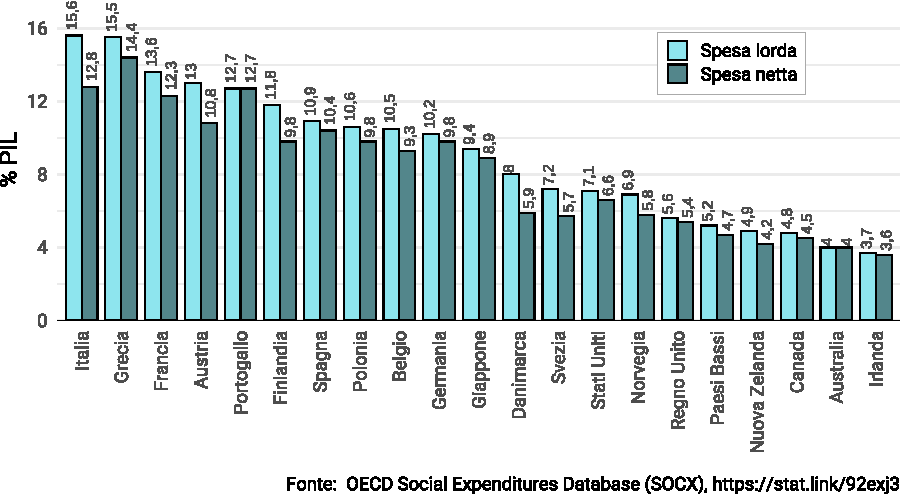
\includegraphics[width=\textwidth]{./figure/pensione-lorda-netta-2017-color.pdf}
\end{figure}
\end{frame}


\section{Gli effetti della spesa pensionistica}

%%%%%%%%%%%%%%%%%%%%%%%%%%%%%%%%%%%%%%%%%%%%%%
\begin{frame}{Dal punto di vista individuale}
\begin{columns}
\begin{column}{.5\columnwidth}
\begin{itemize}
\item La spesa pensionistica è per certi versi analoga al risparmio
\begin{equation*}
\begin{split}
  c^2&=(1+r)\hat{s}+p\\
  &=(1+r)[(1-t)z-c^1]+p
\end{split}
\end{equation*}
per cui, indicando con $\rho$ il rendimento della pensione ($1+\rho = \frac{p}{tz}$):
\begin{equation*}
z-\frac{r-\rho}{1+r}tz=c^1+\frac{c^2}{1+r}
\end{equation*}
\item Possiamo valutare l'effetto redistributivo delle pensioni confrontando
$r$ e $\rho$
\item Equità attuariale quando $\rho=r$
\end{itemize}
\end{column}

\begin{column}{.5\columnwidth}
\begin{figure}[htbp]
\centering
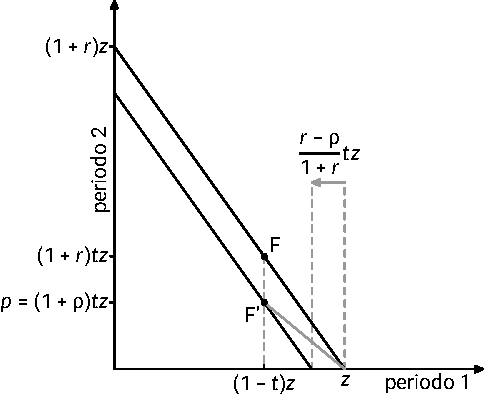
\includegraphics[width=\textwidth]{./figure/effetti-sul-risparmio-0.pdf}
\end{figure}
\end{column}
\end{columns}
\end{frame}

%%%%%%%%%%%%%%%%%%%%%%%%%%%%%%%%%%%%%%%%%%%%%%
\begin{frame}{Effetti redistributivi delle pensioni}
\begin{itemize}
\item La redistribuzione può essere \emph{intergenerazionale} (tra diverse generazioni)
o \emph{intragenerazionale} (tra individui di una stessa generazione).
\item Tra generazioni se un sistema pensionistico garantisce un rendimento $\rho$
diverso da $r$ in media ai membri di una generazione:
\begin{itemize}
\item \alert{effetto prima generazione}.
\end{itemize}
\item Tra gli individui di una stessa generazione si parla di \alert{equità
quasi-attuariale} (ma in alcuni casi si usa «attuariale») se a tutti è
garantito lo stesso rendimento:
\begin{itemize}
\item sistemi contributivi.
\end{itemize}
\end{itemize}
\end{frame}

%%%%%%%%%%%%%%%%%%%%%%%%%%%%%%%%%%%%%%%%%%%%%%
\begin{frame}{L'effetto prima generazione}
\begin{itemize}
\item L'istituzione di un sistema a ripartizione comporta un trasferimento
immediato alla generazione anziana, indipendentemente dal fatto che questa
abbia versato contributi in precedenza
\end{itemize}
\begin{center}
\footnotesize
\begin{center}
\begin{tabular}{lrrrrr}
\hline
ripartizione ($g=0$, $r=0,2$) & 1 & 2 & 3 & 4 & 5\\[0pt]
\hline
reddito dei giovani & 1000 & 1000 & 1000 & 1000 & 1000\\[0pt]
contributi pensionistici & 400 & 400 & 400 & 400 & 400\\[0pt]
consumo dei giovani & 600 & 600 & 600 & 600 & 600\\[0pt]
pensioni/consumo degli anziani & 400 & 400 & 400 & 400 & 400\\[0pt]
\hline
\end{tabular}
\end{center}
\end{center}

\begin{center}
\footnotesize
\begin{center}
\begin{tabular}{lrrrrr}
\hline
capitalizzazione ($g=0$, $r=0,2$) & 1 & 2 & 3 & 4 & 5\\[0pt]
\hline
reddito dei giovani & 1000 & 1000 & 1000 & 1000 & 1000\\[0pt]
contributi pensionistici & 400 & 400 & 400 & 400 & 400\\[0pt]
consumo dei giovani & 600 & 600 & 600 & 600 & 600\\[0pt]
pensioni/consumi degli anziani & 0 & 480 & 480 & 480 & 480\\[0pt]
\hline
\end{tabular}
\end{center}
\end{center}

\begin{itemize}
\item Il guadagno per la prima generazione è pari al valore attuale del costo per le
generazioni future (un gioco a somma zero)
\begin{equation*}
\sum_{t=1}^{\infty}\frac{80}{(1+r)^{t}}=\frac{80}{r}=400
\end{equation*}
\end{itemize}
\end{frame}

%%%%%%%%%%%%%%%%%%%%%%%%%%%%%%%%%%%%%%%%%%%%%%
\begin{frame}{La redistribuzione intergenerazionale}
\begin{itemize}
\item Definiamo l'\alert{imposta implicita} gravante sulla generazione $i$:
\begin{equation*}
\text{imposta implicita} = \frac{r_i-\rho_i}{1+r_i}tz_i.
\end{equation*}

\item Con $\rho=g$ (sistema a ripartizione) e ipotizzando $r_i=r$ costante e
$g_i=g$ costante, per cui $z_{i+1}N_{i+1}=(1+g)z_iN_i$, consideriamo
l'imposta implicita per tutte le generazioni future:
\begin{multline*}
 \frac{r-g}{1+r}tz_1N_1+\frac{1}{1+r}\frac{r-g}{1+r}tz_2N_2+\frac{1}{(1+r)^2}\frac{r-g}{1+r}tz_3N_3+\dots\\
=\frac{r-g}{1+r}tz_1N_1\left[ 1+ \frac{1+g}{1+r} + \frac{(1+g)^2}{(1+r)^2} + \dots \right]\\
=\frac{r-g}{1+r}tz_1N_1\sum_{i=0}^\infty\left(\frac{1+g}{1+r}\right)^i
=\frac{r-g}{1+r}tz_1N_1\frac{1}{1-\dfrac{1+g}{1+r}} =tz_1N_1.
\end{multline*}
\item L'ammontare complessivo attualizzato delle imposte implicite è pari a
$tz_1N_1$, la somma dei contributi versati nel periodo corrente, che a sua
volta è pari all'ammontare delle pensioni dovute ai pensionati attuali.
\end{itemize}
\end{frame}

%%%%%%%%%%%%%%%%%%%%%%%%%%%%%%%%%%%%%%%%%%%%%%
\begin{frame}{Inefficienza/Efficienza dinamica}
\begin{itemize}
\item Si dice che un'economia è \alert{dinamicamente inefficiente} quando $g>r$. Se
$n+m=g>r$ è infatti possibile realizzare un miglioramento paretiano per
tutte le generazioni attraverso un sistema a ripartizione.
\item Vediamo come:
\begin{itemize}
\item assumiamo per semplicità $m=0$, per cui $g=n$;
\item ipotizziamo di introdurre un trasferimento dai giovani agli anziani: per
ogni euro prelevato dai giovani abbiamo $1+n$ euro per gli anziani;
\item se a seguito del prelievo i giovani riducono i risparmi di un euro, il
loro consumo da giovani non varia, mentre il loro consumo da vecchi varia
di $(1+n)-(1+r)=n-r$;
\item se $n>r$ c'è un vantaggio per tutte le generazioni (miglioramento
paretiano);
\item se $n<r$ c'è un vantaggio per la prima generazione (gli anziani di oggi)
che costa $r-n$ alle generazioni successive.
\end{itemize}
\item L'opinione prevalente è che tutte le maggiori economie siano in condizioni
di efficienza dinamica ($g<r$), ma in passato, nei periodi di crescita più
rapida, si è verificato il caso di $g>r$
\end{itemize}
\end{frame}

%%%%%%%%%%%%%%%%%%%%%%%%%%%%%%%%%%%%%%%%%%%%%%
\begin{frame}{Inefficienza/Efficienza dinamica /2}
Illustriamo quanto detto nella slide precedente:
\begin{itemize}
\item la generazione $t$ lavora nel periodo $t$ e si gode la pensione e i risparmi
nel periodo $t+1$
\item includiamo nel prospetto la generazione 0, che è già in pensione al momento
in cui il trasferimento viene introdotto
\item ipotizziamo un trasferimento di un euro e una riduzione del risparmio di un
euro, per cui il consumo degli attivi non varia
\end{itemize}
\begin{center}
\footnotesize
\begin{center}
\begin{tabular}{llllrr}
\hline
periodi & 1 & 2 & 3 & 4 & 5\\[0pt]
\hline
generazione 0 & $1+n$ &  &  &  & \\[0pt]
generazione 1 & $1-1$ & $n-r$ &  &  & \\[0pt]
generazione 2 &  & $1-1$ & $n-r$ &  & \\[0pt]
generazione 3 &  &  & $1-1$ & $n-r$ & \\[0pt]
generazione 4 &  &  &  & $1-1$ & $n-r$\\[0pt]
\ldots{} &  &  &  &  & \ldots{}\\[0pt]
\hline
\end{tabular}
\end{center}
\end{center}
\begin{itemize}
\item il prospetto evidenzia un "effetto prima generazione"
\end{itemize}
\end{frame}

%%%%%%%%%%%%%%%%%%%%%%%%%%%%%%%%%%%%%%%%%%%%%%
\begin{frame}{Gli effetti della pensione sul risparmio}
\begin{columns}
\begin{column}{.5\columnwidth}
\begin{itemize}
\item Se il risparmio serve a finanziare i consumi in età anziana (teoria del
ciclo vitale) la pensione determina uno «spiazzamento» del risparmio
volontario, che si riduce in modo corrispondente
\item Quando $\rho=r$ (capitalizzazione oppure ripartizione con $g=r$) lo
spiazzamento è totale
\end{itemize}
\end{column}

\begin{column}{.5\columnwidth}
\begin{figure}[htbp]
\centering
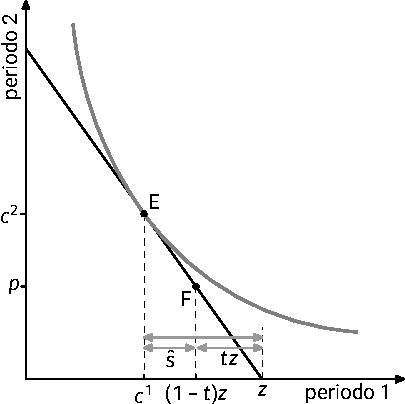
\includegraphics[width=\textwidth]{./figure/effetti-sul-risparmio-2.pdf}
\end{figure}
\end{column}
\end{columns}
\end{frame}

%%%%%%%%%%%%%%%%%%%%%%%%%%%%%%%%%%%%%%%%%%%%%%
\begin{frame}{Gli effetti della pensione sul risparmio /2}

\begin{columns}
\begin{column}{.5\columnwidth}
\begin{itemize}
\item Se i contributi pensionistici ($tz$) eccedono il livello di risparmio
desiderato e l'individuo ha accesso al credito, è possibile un risparmio
negativo $\hat s<0$;
\item l'equilibrio è comunque E.
\end{itemize}
\end{column}

\begin{column}{.5\columnwidth}
\begin{center}
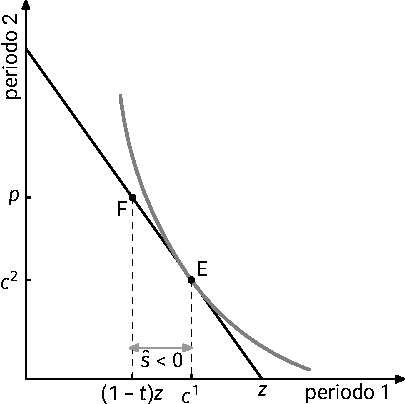
\includegraphics[width=\linewidth]{./figure/effetti-sul-risparmio-3.pdf}
\end{center}
\end{column}
\end{columns}
\end{frame}


%%%%%%%%%%%%%%%%%%%%%%%%%%%%%%%%%%%%%%%%%%%%%%
\begin{frame}{Gli effetti della pensione sul risparmio /3}

\begin{columns}
\begin{column}{.5\columnwidth}
\begin{itemize}
\item Se invece un risparmio negativo ($\hat s<0$) non è possibile perché
  l'individuo non ha la possibilità di indebitarsi, la pensione porta a un
  aumento del risparmio.
\item L'individuo può percepire tale aumento forzato del risparmio come una
riduzione di utilità.
\item Nota bene: qui stiamo ipotizzando un \alert{individuo pienamente razionale e
lungimirante}. Ma sotto tale ipotesi l'esistenza di un sistema pensionistico
non trova giustificazione\ldots{}
\end{itemize}
\end{column}

\begin{column}{.5\columnwidth}
\begin{center}
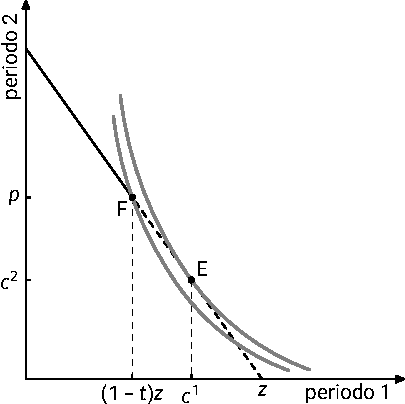
\includegraphics[width=\linewidth]{./figure/effetti-sul-risparmio-4.pdf}
\end{center}
\end{column}
\end{columns}
\end{frame}


%%%%%%%%%%%%%%%%%%%%%%%%%%%%%%%%%%%%%%%%%%%%%%
\begin{frame}{Gli effetti della pensione sul risparmio /3}
\begin{columns}
\begin{column}{.5\columnwidth}
\begin{itemize}
\item Nel caso in cui $\rho<r$ (ad esempio con un sistema a ripartizione se $g<r$)
si determina una riduzione del reddito dell'individuo nel corso della vita.
\item L'effetto è uno spiazzamento non completo del risparmio: il risparmio
complessivo dell'individuo aumenta
\item (il caso con contributi superiori al livello di risparmio desiderato è
lasciato come esercizio)
\end{itemize}
\end{column}

\begin{column}{.5\columnwidth}
\begin{figure}[htbp]
\centering
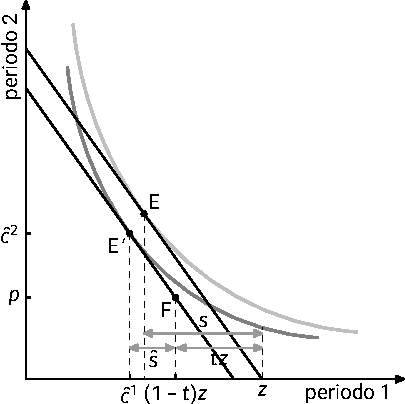
\includegraphics[width=\textwidth]{./figure/effetti-sul-risparmio-5.pdf}
\end{figure}
\end{column}
\end{columns}
\end{frame}

%%%%%%%%%%%%%%%%%%%%%%%%%%%%%%%%%%%%%%%%%%%%%%
\begin{frame}{Gli effetti sul risparmio aggregato}
\begin{itemize}
\item In assenza di un sistema pensionistico, indicando con $s$ la quota di
reddito risparmiata:
\begin{itemize}
\item il risparmio complessivo della generazione $i$ di giovani è $N_isz_i$
\item nel periodo successivo, tale risparmio viene decumulato e va sottratto al
risparmio dei giovani della generazione $i+1$:
\begin{equation*}
\begin{split}
sz_{i+1}N_{i+1}-sz_iN_i&=\left(1-\frac{1}{1+g_i}\right)sz_{i+1}N_{i+1} \\
&= \frac{g_i}{1+g_i}sz_{i+1}N_{i+1}.
\end{split}
\end{equation*}
\item il risparmio è positivo se e solo se $g_i>0$
\end{itemize}
\item Il sistema pensionistico determina uno spiazzamento del risparmio, tuttavia:
\begin{itemize}
\item con la capitalizzazione il risparmio pensionistico rappresenta risparmio
\item con la ripartizione, il risparmio pensionistico è consumato dagli anziani,
dunque la quota di risparmio è solo quella volontaria $\hat s$.
\end{itemize}
\end{itemize}
\end{frame}


%%%%%%%%%%%%%%%%%%%%%%%%%%%%%%%%%%%%%%%%%%%%%%
\begin{frame}{Gli effetti sul risparmio: in conclusione}
\begin{itemize}
\item Il sistema pensionistico determina uno spiazzamento del risparmio
volontario, un aumento nei casi in cui l'individuo non può compensare
indebitandosi.
\item La differenza tra capitalizzazione e ripartizione è che nel primo caso il
risparmio pensionistico è risparmiato e diventa risparmio negativo nel
periodo successivo, nel secondo caso è consumato immediatamente dagli
anziani.
\item La conclusione nel modello economico neoclassico è che con la
capitalizzazione il livello di risparmio aggregato è superiore che con la
ripartizione.
\begin{itemize}
\item Nella misura in cui il risparmio aumenta l'investimento, questo è un
argomento a favore della capitalizzazione.
\item Ulteriore effetto positivo: i fondi pensione, investitori con orientamento
a lungo termine, conferiscono stabilità ai mercati finanziari.
\end{itemize}
\end{itemize}
\end{frame}

%%%%%%%%%%%%%%%%%%%%%%%%%%%%%%%%%%%%%%%%%%%%%%
\begin{frame}{I contributi pensionistici}
\begin{center}
\begin{tabular}{lccc}
    \toprule
    &A carico del&A carico del&\\[-1mm]
    &lavoratore&datore di lavoro&Totali\\
    \midrule
    Austria* &10,25 &12,55 &22,8\\
    Belgio &7,5 &8,9 &16,4\\
    Francia** &11,3 &16,5 &27,8\\
    Germania* &9,3 &9,3 &18,6\\
    Grecia &6,7 &19,8 &26,5\\
    Italia* &9,19 &23,81 &33,0\\
    Norvegia &8,2 &15,0 &23,2\\
    Polonia &9,8 &9,8 &19,5\\
    Portogallo &7,2 &15,5 &22,7\\
  \bottomrule
\multicolumn{4}{l}{\scriptsize * Finanziano anche le pensioni di invalidità.}\\[-5pt]  
\multicolumn{4}{l}{\scriptsize ** Variano al variare della retribuzione.}\\
\multicolumn{4}{r}{\scriptsize Fonte: OECD, \emph{Pensions at a Glance 2022}, Table 8.1.}\\  
  \end{tabular}
\end{center}
\end{frame}

%%%%%%%%%%%%%%%%%%%%%%%%%%%%%%%%%%%%%%%%%%%%%%
\begin{frame}{I contributi pensionistici in Italia}
\begin{center}\small
\begin{tabular}{lrr}
\toprule
Contributi al fondo pensioni: && 33,00 \\
\qquad di cui a carico del datore di lavoro: & 23,81 &\\
\qquad di cui a carico del lavoratore: & 9,19 &\\
Altri contributi a carico del datore di lavoro:* && 8,07 \\
Altri contributi a carico del lavoratore:* && 0,30 \\
\bottomrule\footnotesize * percentuali variabili per settore e tipologia di contratto&&\\
\end{tabular}
\end{center}

Calcoliamo dunque il costo del lavoro: $100 + 23,81 + 8,07 = 132,08$.

L'incidenza complessiva dei contributi pensionistici rapportata al
costo del lavoro è dunque: $33/132,08 = 24,98\%$. Il reddito imponibile al netto dei contributi è: $100 - 9,19 - 0,30 = 90,51$.

\alert{I contributi sono imposte o reddito differito?}
\end{frame}

%%%%%%%%%%%%%%%%%%%%%%%%%%%%%%%%%%%%%%%%%%%%%%
\begin{frame}{Gli effetti sull'incentivo al lavoro}
\begin{itemize}
\item I contributi pensionistici sono una forma di prelievo fiscale. Le imposte
determinano un incentivo al lavoro in quanto un incremento del reddito lordo
$\Delta z$ si traduce in un aumento di consumo $(1-t)\Delta z$
\item Tuttavia, a differenza delle imposte, ai contributi pensionistici sono
collegate le prestazioni. Bisogna tenere conto degli effetti \alert{al margine}
sull'intero vincolo di bilancio dell'individuo.
\item L'effetto sul bilancio di un aumento del reddito è:
\begin{equation*}
  (1-t)\Delta z +\frac{\Delta p}{1+r} 
\end{equation*}
\item L'effetto sull'incentivo al lavoro dipende da $\Delta p/\Delta z$.
\item Se c'è equità attuariale, $\Delta p=(1+r)t\Delta z$. L'espressione si riduce
a $\Delta z$. I contributi sono assimilabili a \alert{reddito differito}.
\end{itemize}
\end{frame}


%%%%%%%%%%%%%%%%%%%%%%%%%%%%%%%%%%%%%%%%%%%%%%
\begin{frame}{Gli effetti sull'incentivo al lavoro /2}
\begin{itemize}
\item Con pensione di base $\Delta p=0$, per cui i contributi sono assimiliabili a
imposta.
\item Con metodo contributivo $\Delta p = (1+g)t\Delta z$ («quasi-equità
attuariale»), per cui
\begin{equation*}
  (1-t)\Delta z +\frac{(1+g)t\Delta z}{1+r}.
\end{equation*}
se $g=r$ assimilabile a reddito differito, con $g<r$ è in parte come
un'imposta
\item Con prestazione definita (retributivo): più complesso, nelle fasi iniziali
della carriera simile a imposta, nelle fasi finali può addirittura avere un
effetto incentivante
\end{itemize}
\end{frame}


\section{Le riforme dei sistemi pensionistici}

%%%%%%%%%%%%%%%%%%%%%%%%%%%%%%%%%%%%%%%%%%%%%%
\begin{frame}{Vari tipi di shock possono destabilizzare i sistemi pensionistici}
\begin{itemize}
\item I diversi schemi pensionistici reagiscono diversamente ai possibili shock.
\begin{itemize}
\item Shock di natura finanziaria
\item Shock «politici»
\item Shock relativi all'andamento economico e demografico
\end{itemize}
\end{itemize}

\begin{figure}[htbp]
\centering
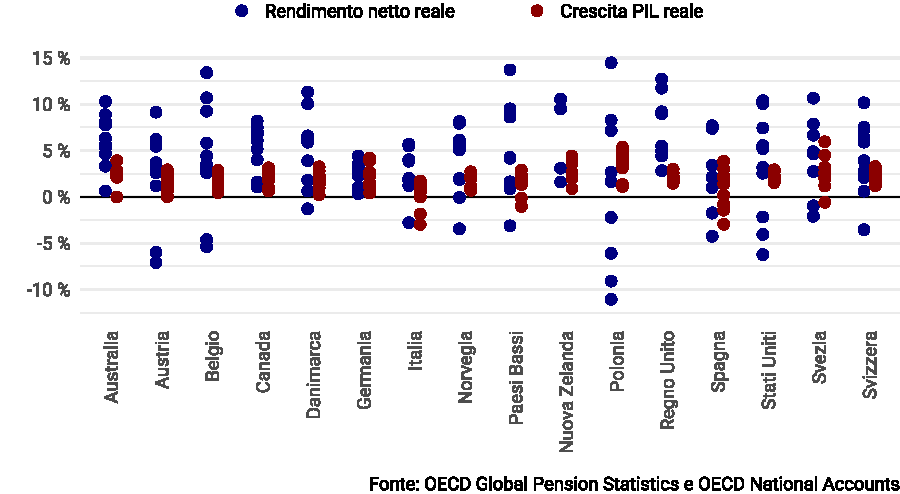
\includegraphics[height=5.5cm]{./figure/crescita-e-rendimenti-2010-2019-color.pdf}
\end{figure}
\end{frame}

%%%%%%%%%%%%%%%%%%%%%%%%%%%%%%%%%%%%%%%%%%%%%%
\begin{frame}{Rischio politico}
\begin{itemize}
\item Garantisce di più l'esistenza di un fondo di attività finanziarie o una
promessa dello Stato?

\begin{quoting}
«[L]’esistenza di riserva, più che costituire una garanzia
fornita addizionale a favore dei beneficiari, fa non irragionevolmente
sorgere il timore che essa venga ritorta a danno di essi, invocandosi
l’insufficienza (causa svalutazioni o altri fattori) dei fondi accumulati a
titolo di garanzia, quale motivo per annullare l’obbligazione sostanziale al
sostentamento degli
individui trovatisi nelle condizioni debite.» (Bruno De Finetti, 1956)
\end{quoting}

\item Rischio di modifica unilaterale dei termini della promessa
\item Rischio di espropriazione del valore del fondo attraverso politiche
monetarie o anche interventi diretti
\end{itemize}
\end{frame}

%%%%%%%%%%%%%%%%%%%%%%%%%%%%%%%%%%%%%%%%%%%%%%
\begin{frame}{Rischi di natura economica/demografica}
\begin{equation*}
  \frac{\text{SP}}{\text{PIL}} =\frac{\dfrac{\text{SP}}{N_P}\,\dfrac{N_P}{N_A}\,\dfrac{N_A}{N_G}\,}
  {\dfrac{\text{PIL}}{N_L}\,\dfrac{N_L}{N_G}}
\end{equation*}

\begin{itemize}
\item Dove:
\begin{itemize}
\item $N_P$ = numero di pensionati
\item $N_A$ = numero di anziani (a prescindere dal fatto che percepiscano o meno una pensione)
\item $N_G$ è la popolazione in età lavorativa
\item $N_L$ è il numero di coloro che sono effettivamente attivi.
\end{itemize}
\item Dunque:
\begin{itemize}
\item SP$/N_P$ = pensione media corrisposta ai pensionati;
\item $N_P/N_A$ = estensione del diritto pensionistico;
\item $N_A/N_G$ = indice di dipendenza (\emph{old age dependency ratio})
\item $N_L/N_G$ = tasso di attività
\item $\text{PIL}/N_L$ = produttività media del lavoro
\end{itemize}
\end{itemize}
\end{frame}


%%%%%%%%%%%%%%%%%%%%%%%%%%%%%%%%%%%%%%%%%%%%%%
\begin{frame}{Il tasso di dipendenza  (\emph{old age dependency ratio})}
\begin{figure}[htbp]
\centering
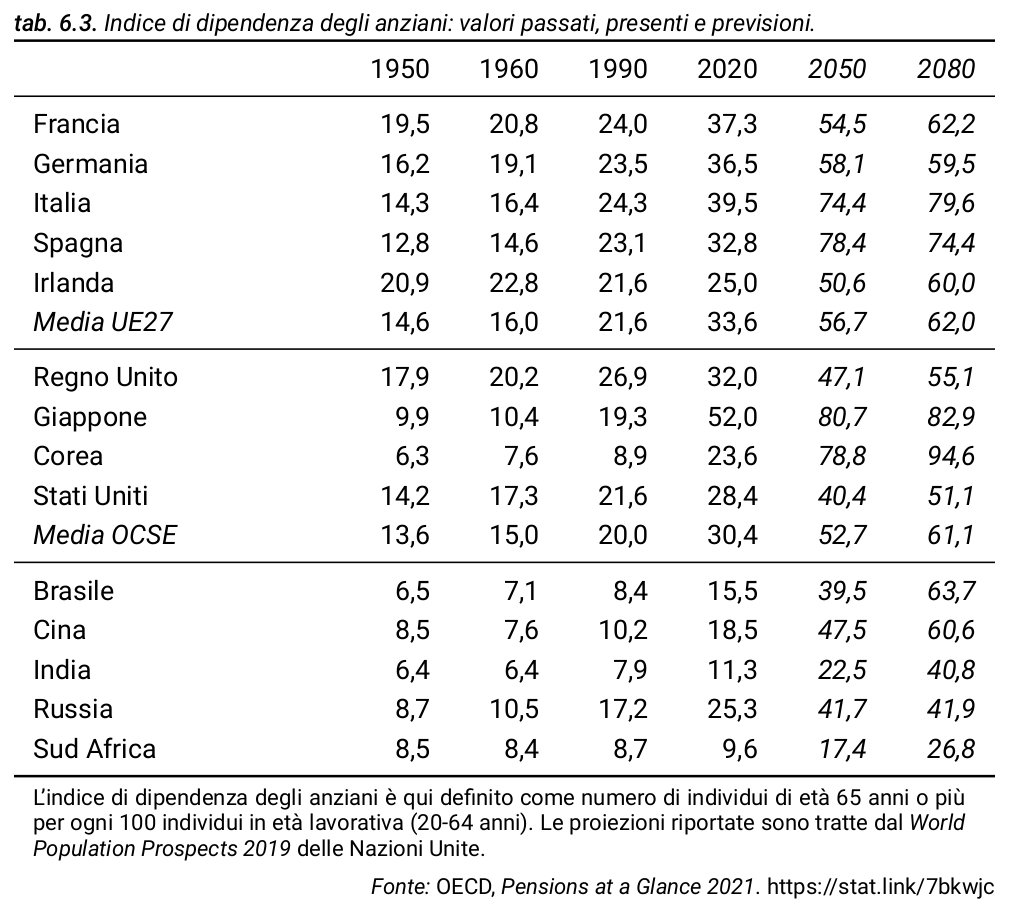
\includegraphics[height=8cm]{./figure/old-age-dependency-ratio.png}
\end{figure}
\end{frame}


%%%%%%%%%%%%%%%%%%%%%%%%%%%%%%%%%%%%%%%%%%%%%%
\begin{frame}{Misure di contrasto alla crescita della spesa pensionistica}
\begin{itemize}
\item Innalzamento dell'età pensionabile, dovuta a interventi \emph{ad hoc} o prevista
attraverso adeguamenti programmati dei parametri
\item Agisce riducendo $N_P/N_A$ e aumentando $N_L/N_G$
\end{itemize}

\begin{figure}[htbp]
\centering
\includegraphics[height=6.5cm]{./figure/evoluzione-età-pensionabile.png}
\end{figure}
\end{frame}


%%%%%%%%%%%%%%%%%%%%%%%%%%%%%%%%%%%%%%%%%%%%%%
\begin{frame}{Andamento dell'età effettiva di pensionamento}
\begin{figure}[htbp]
\centering
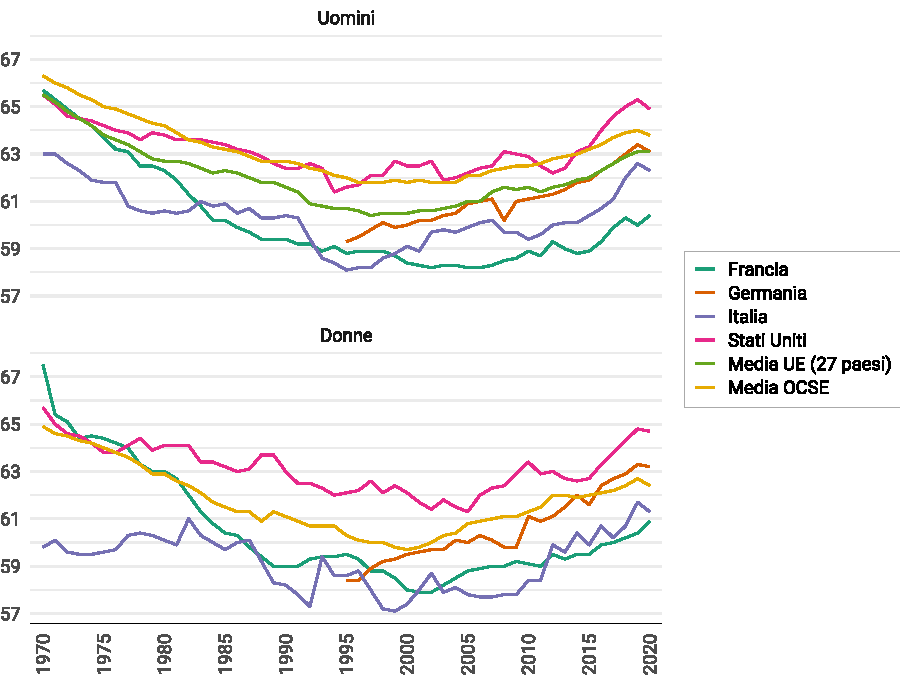
\includegraphics[height=7cm]{./figure/eta-effettiva-pensionamento-color.pdf}
\end{figure}
\end{frame}

%%%%%%%%%%%%%%%%%%%%%%%%%%%%%%%%%%%%%%%%%%%%%%
\begin{frame}{Riduzione delle prestazioni}
\begin{itemize}
\item Requisiti più stringenti per la pensione e modifica dei parametri che
determinano il loro ammontare (compresa l'indicizzazione all'inflazione)
\item Il sistema contributivo prevede dei meccanismi di aggiustamento automatico
\begin{itemize}
\item il tasso di rendimento (usato per calcolare il montante) segue la crescita
\item la pensione viene "aggiustata" in base all'aumento della speranza di vita
\end{itemize}
\end{itemize}

\begin{figure}[htbp]
\centering
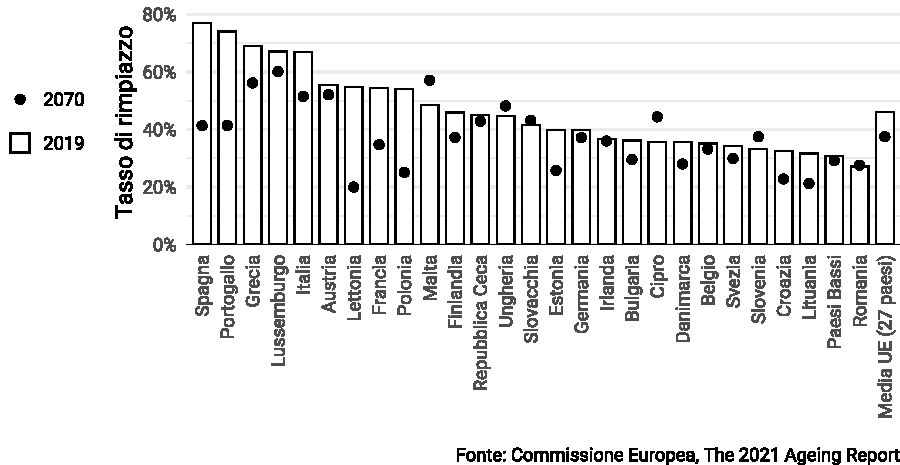
\includegraphics[height=5.5cm]{./figure/tassi-rimpiazzo-2019-2070.pdf}
\end{figure}
\end{frame}

%%%%%%%%%%%%%%%%%%%%%%%%%%%%%%%%%%%%%%%%%%%%%%
\begin{frame}{Altri possibili interventi di politica economica}
Altri interventi, non relativi specificamente alle pensioni, possono incidere sulla sostenibilità di un sistema pensionistico: 
\begin{itemize}
\item L'aumento del tasso di attività
\item L'aumento della natalità
\item L'immigrazione
\item \ldots{}e naturalmente la crescita economica!
\end{itemize}
\end{frame}

%%%%%%%%%%%%%%%%%%%%%%%%%%%%%%%%%%%%%%%%%%%%%%
\begin{frame}{Ipotesi più radicali di riforma: il passaggio alla capitalizzazione}
\begin{itemize}
\item Si ritiene che la capitalizzazione sia meglio attrezzata rispetto alle
variazioni demografiche:
\begin{itemize}
\item meno vulnerabile del sistema a ripartizione rispetto agli shock
demografici
\item incoraggia il risparmio
\item fornisce rendimenti più alti ($r>g$)
\end{itemize}
\item La ricetta del \emph{«Washington consensus»} degli anni Novanta, che ha
influenzato molti paesi, specialmente emergenti:
\begin{itemize}
\item capitalizzazione
\item formule di calcolo a contribuzione definita che realizzino l'equità
attuariale
\item gestione privata dei fondi pensione
\end{itemize}
\end{itemize}
\end{frame}

%%%%%%%%%%%%%%%%%%%%%%%%%%%%%%%%%%%%%%%%%%%%%%
\begin{frame}{I sistemi a capitalizzazione e la demografia}
\begin{itemize}
\item È proprio vero che i sistemi a capitalizzazione non risentono degli effetti
demografici?
\begin{itemize}
\item I prezzi di mercato «aggiustano» i valori delle attività accumulate e
risentono dello squilibrio demografico tra giovani e anziani (un
«vantaggio» è che gli aggiustamento sono attuati dal mercato e questo può
ridurne il costo politico)
\item In ultima analisi, il problema demografico dipende dalla disponibilità di
risorse, non dal particolare meccanismo con il quale tale risorse sono
allocate tra popolazione attiva e pensionati (Barr e Diamond, 2006).
\end{itemize}
\item Il sistema a capitalizzazione viene considerato superiore perché incoraggia
il risparmio e quindi l'accumulazione di capitale, che aumenta le risorse
disponibili. Tuttavia
\begin{itemize}
\item aumentare il risparmio significa ridurre i consumi nella fase di
transizione (se invece c'è spiazzamento del risparmio volontario o del
risparmio pubblico\ldots{})
\item in ottica keynesiana, non è detto che aumentare il risparmio aumenti
l'accumulazione
\end{itemize}
\item Anche concludendo che il sistema a capitalizzazione è preferibile perché il
rendimento è più elevato, resta il problema della \alert{transizione}
\end{itemize}
\end{frame}

%%%%%%%%%%%%%%%%%%%%%%%%%%%%%%%%%%%%%%%%%%%%%%
\begin{frame}{Il problema della transizione}
\begin{figure}[htbp]
\centering
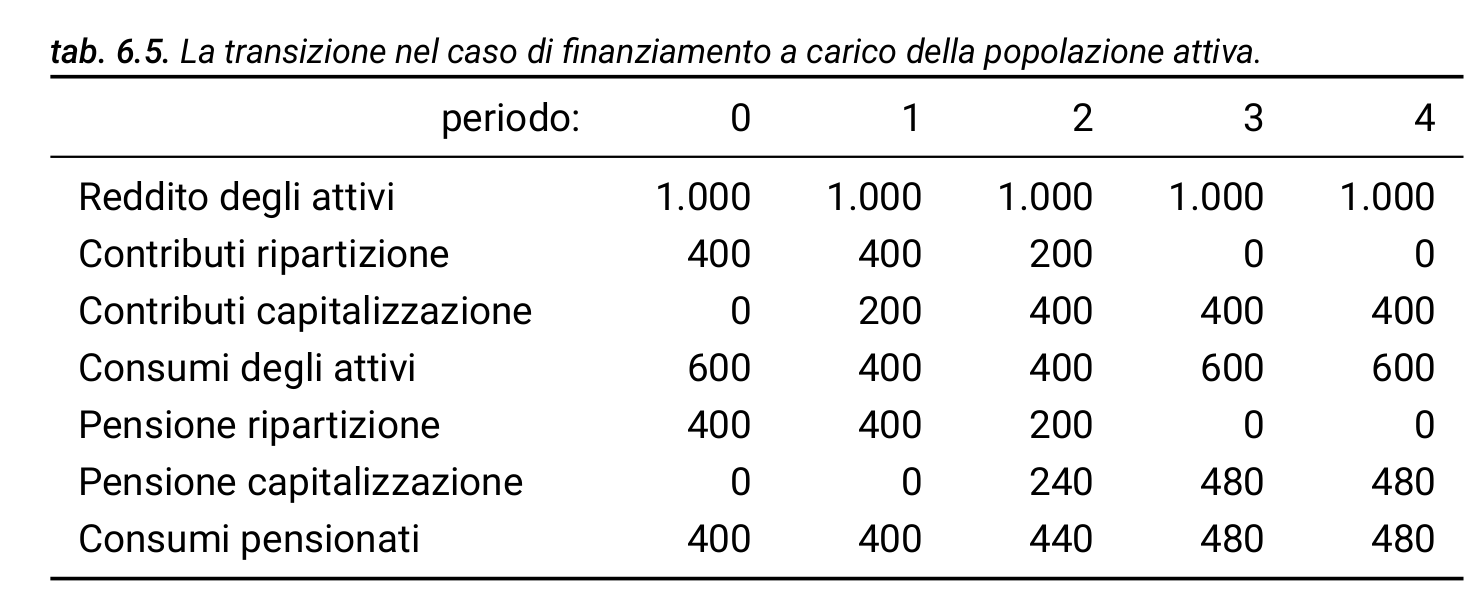
\includegraphics[width=\textwidth]{./figure/transizione-alla-capitalizzazione-1.png}
\end{figure}
\end{frame}


%%%%%%%%%%%%%%%%%%%%%%%%%%%%%%%%%%%%%%%%%%%%%%
\begin{frame}{Il problema della transizione /2}
\begin{figure}[htbp]
\centering
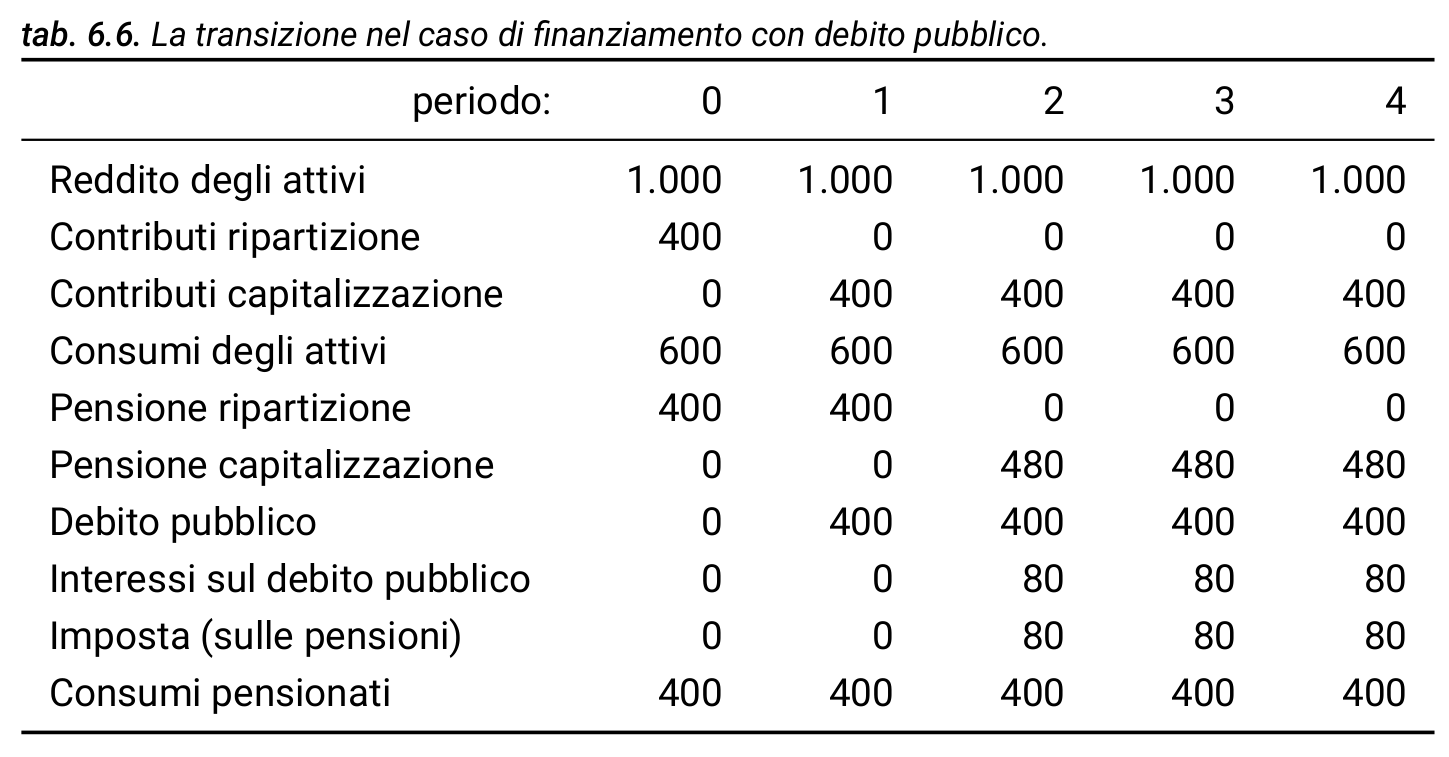
\includegraphics[width=\textwidth]{./figure/transizione-alla-capitalizzazione-2.png}
\end{figure}
\end{frame}
\end{document}
